% Chapter 2

\chapter{Background} % Main chapter title

\label{Chapter2} % For referencing the chapter elsewhere, use \ref{Chapter2} 


%----------------------------------------------------------------------------------------

\section{Reinforcement Learning}
\label{RL}

\subsection{Markov Decision Processes}
\label{MDP}
Environments in traditional reinforcement learning application are usually modelled as Markov Decision Processes or MDPs.

These can be formulated as systems with the following components:
\begin{itemize}
	\item Finite set of states $S=\{s_0,\ldots,s_n\}$ and actions $A=\{a_0,\ldots,a_m\}$.
	\item A distribution of probabilities $P_a(s,s')$ for transitions from state $s$ to $s'$ for each possible action $a$.
	\item A reward function $R:S\mapsto\mathbb{R}$ for being at a particular state.
	\item The goal in reinforcement learning is to maximise the final reward that an agent achieves in the environment.
\end{itemize}

As the name suggests, MDPs obey the \textit{Markov property}, whereby the probability of the system being in a certain future state exclusively depends upon the present state, and not upon an arbitrarily-long sequence of past states.

In figure~\ref{fig:MDP} we show a sample schematic of a Markov Decision Process, and how states, actions, and rewards could be connected between each other.

\begin{figure}
\centering
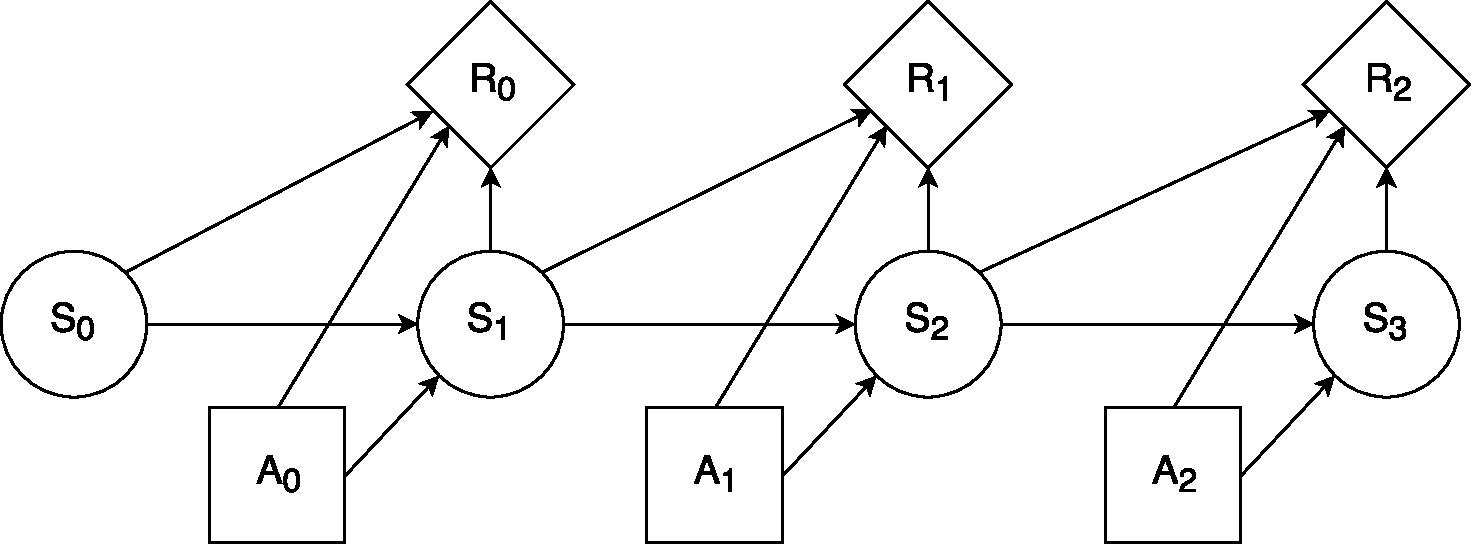
\includegraphics[width=10cm]{Figures/MDP}
\caption{Sample schematic of an MDP.}
\label{fig:MDP}
\end{figure}


\subsection{Q-learning}
\label{qlearning}
Now that we contextualised reinforcement learning environments as Markov Decision Processes, we can introduce the final objective of reinforcement learning tasks: finding a function $\Pi:S\mapsto A$ called \textbf{policy}, that maps the appropriate action $a\in A$ given the current state $s\in S$, as to maximise our agent's final reward.

In particular, we will now present Q-learning \parencite{watkins1992q}, an algorithm that yields an optimal policy given an MDP.

Q-learning lets us learn the \emph{quality}, or expected utility, for each state-action combination. That is, for each state, let's estimate all the expected rewards we obtain by taking each possible action at that particular state.

More formally, we estimate a function $Q: S \times A \to \mathbb{R}$. We can model $Q$ as a mapping table (initialised with some uniform values), whose value we update at each time step of our simulations.

Here's how we update our Q-table at each time step $t$:
  \[Q(s_{t},a_{t}) = \underbrace{Q(s_t,a_t)}_{\rm old~value} +
  \underbrace{\alpha}_{\rm learning~rate} \times \left[
    \overbrace{\underbrace{r_{t+1}}_{\rm reward} + \underbrace{\gamma}_{\rm
        discount~factor} \underbrace{\max_{a}Q(s_{t+1}, a)}_{\rm
        estimate~of~optimal~future~value}}^{\rm learned~value} -
    \underbrace{Q(s_t,a_t)}_{\rm old~value} \right] \]
    
where:
\begin{itemize}
	\item $\alpha\in[0,1]$ is the \emph{learning rate}, a coefficient that regulates how much the newly learned values will contribute in the update
	\item $\gamma\in[0,1]$ is the \emph{discount factor}, a coefficient that controls the weight of future rewards. Values closer to 0 will make our agent "short-sighted", considering only the immediate rewards.
\end{itemize}

What is our optimal policy when we do Q-learning then? After training, it is simply that function $\pi: S \to A$ that, for each state, returns the action with maximum expected utility in our Q-table.

\subsection{Exploration/Exploitation tradeoff}
An important theme in reinforcement learning, and that we heavily focus our attention on in our project is the idea of the tradeoff between Exploration and Exploitation.

\subsection{Deep Reinforcement Learning}
\subsubsection{DQGAN}
\subsection{Problems with reinforcement learning techniques}
\subsection{Actor critic}

%----------------------------------------------------------------------------------------

\section{Generative Adversarial Networks}
\subsection{Architecture of GANs}
\subsection{Successes}
\label{successes}
\subsubsection{DCGAN}
\subsection{Conditional GANs}

%----------------------------------------------------------------------------------------

\section{Existing related work}
\subsection{Generative Adversarial Imitation Learning}

%----------------------------------------------------------------------------------------